\documentclass{article}
\usepackage[utf8]{inputenc}
\usepackage[ngerman]{babel}
\usepackage{enumitem}
\usepackage{graphicx}
\usepackage{amsmath}
\usepackage[version=3]{mhchem} 		%% \ce{CO2} -- automatische subscript der zahlen
\usepackage{booktabs}
\usepackage{subfig}
\usepackage{textcomp}
\usepackage{multirow}
\usepackage{fixltx2e}
\usepackage{natbib}
\usepackage{color}

\begin{document}
\title{Kleines Script zur Mikrobiologieklausur}
\author{Christian Müller}

\pagestyle{empty}
\maketitle
\tableofcontents

\pagestyle{headings}
\newpage
\section{Stoffwechsel}
\subsection{Phototrophie}
\begin{description}
	\item[ATP-Produktion]	\hfill \\
	\item[Reduktion von Kohlenstoffdioxid]	\hfill	\\
		mit \ce{NADH} und \ce{NADPH},
		welche durch die vorherige Reduktion von \ce{NAD+} bzw. \ce{NADP*} erzeugt wurden.
\end{description}
	Bei beiden Photosynthesevarianten finden
	verschiedener akzessorischer Proteine und Photosystheme verwendung.
	Dies ermöglich die Anpassung an verschiedene Lebensräume,
	und die Anpassung an die vorhanden Lichtspektren.

\subsubsection{Oxygenen Photosynthese}
	\begin{itemize}
		\item Kein zyklischer Elektronen Transport
		\item Z-Schema mit zwei Photosysteme, (II:P680;I:P700)
	\end{itemize}

\subsubsection{Anoxygene Photosynthese}
	\begin{itemize}
		\item zyklischer Elektronen Transport
		\item Ein Photosystem (P870)
		\item umgekehrter, energieverbrauchender Elektronentransport,
			wenn \ce{NAD(P)H} nötig
	\end{itemize}

\subsubsection{\ce{CO2}-Fixierung}
\begin{description}
	\item[Calvin-Zyklus] ist am weitesten verbreitet.
		Mit den Schlüsselenzymen RUBISCO und Phosphoribulose-Kinase
		erfolgt die Bindung von \ce{CO2} in Glucose
		unter Verbrauch von \ce{ATP} und \ce{NADPH}.
		Siehe Abbildung \ref{fig:calvin_detail}.

	\item[Hydroxypropionat-Weg] der Grünen-Schwefelbakterien.
		Letzlich wird in zwei Zyklen zunächst zwei Moleküle \ce{CO2}
		in Form von Bicarbonat (\ce{HCO3-}) fetgelegt.
		Das Bicarbonat wird dann unter ATP und NADPH Verbrauch zu Glyoxalat aufgebaut.

		Anschließend werden zwei Glyoxalat Moleküle zu Pyruvat umgebaut.

	\item[umgekehrter Citrat-Zyklus] ist die Umkehrung des oxidativen Citratzyklus,
		deshalb auch reduktiver Citrat-Zyklus.
		Die Reaktionen innerhalb des oxidativen Zyklus werden dabei umgekehrt
		unter Umgehung bzw. der Verwenugn spezialisierter Moleküle für die 
		drei Unumkerhbahren Schritte des oxidativen Citrat-Zyklus.

\end{description}

\newpage
\section{Begriffe}

%TODO Verweise auf die Sektionen

\begin{description}
	\item[aerob/anaerob]\hfill \\
		Abhängigkeit des Stoffwechsels von Sauerstoff.

	\item[Autotrophie] \hfill \\
		\ce{CO2} als Quelle für Kohlenstoff.
		(Auch: Primäproduzenten)

	\item[Chemolithotrophie]\hfill \\
		Energiegewinnung aus Oxidation anorganischer Substanzen.
		Nur bei Prokaryoten.
		(Auch: Chemoautotrophie)\\
		Beispielsweise: \textbf{\ce{H2}} + \ce{O2} \textrightarrow  \ce{H2O} + \textbf{ATP}

	\item[Chemoorganotrophie]\hfill \\
		Energirgewinnung aus Oxidation organischer Stoffe.\\
		Beispielsweise: \textbf{Glucose} + \ce{O2} \textrightarrow  \ce{CO2} + \ce{H2O} + \textbf{ATP}

	\item[Fermentation] \hfill \\
		Anaerober Katabolismus, bei dem eine organische Verbindung sowohl
		Elektronendonator als auch Elektronenakzeptor dient und bei dem
		ATP durch Substratkettenphosphrylierung gebildet wird.

	\item[Glykolyse] \hfill \\
		Ein biochemischer Weg,
		bei dem Glucose fermentiert wird und ATP sowie verschiedenen
		Fermentationsprodukte gebildet werden.
		(Auch: ``Embden-Myerof-Weg'')

	\item[Heterotrophie] \hfill \\
		Abhängigkeit von mehrern Kohlenstoffquellen.
		Zumeist Chemolithotrophe.

	\item[Oxidationsstufen] \hfill \\
		\begin{table}[h!]
		\begin{center}
		\begin{tabular}{l l} 
			\toprule
			Element			&	Summenformel		\\
			\midrule
			\multicolumn{2}{l}{Schwefel}			\\
			Sulfid			&	\ce{S}$^{2-}$		\\
			Sulfit			&	\ce{SO3}$^{2-}$	\\
			Sulfat			&	\ce{SO4}$^{2-}$	\\
			Thiosulfat		&	\ce{S2O3}$^{2-}$	\\
			\midrule
			\multicolumn{2}{l}{Stickstoff}		\\
			Nitrit			&	\ce{NO2}$^{-}$		\\
			Nitrat			&	\ce{NO3}$^{-}$		\\
			\bottomrule
		\end{tabular}
		\caption{Übersicht über die Oxidationsstufen von Schwefel.}
		\label{tab:oxidationsstufen}
		\end{center}
		\end{table}

	\item[oxidative Poshorylierung] \hfill \\
		Bildung von ATP auf Kosten der protonenmotorischen Kraft,
		die durch Elektronentransport erzeugt wird.

	\item[Photophosphorylierung] \hfill \\
		Bildung von ATP durch die protonenmotorische Kraft,
		die durch lichtangetrieben Elektronentransport erzeugt wird.

	\item[Phototrophie]\hfill \\
		Energirgewinnung durch Licht.\\
		Bei der Oxgenen Photosynthese endsteht Sauerstoff als Abfallprodukt,
		bei der Anoxygenen nicht.
		Phototrophe Organismen sind meinst auch Autotroph.
		Licht \textrightarrow ATP

	\item[protonenmotorische Kraft] 	\hfill	\
		Ein energetisierter Zustand der Membran,
		der durch die Trennung von Ladung und den Elelemten des Wassers
		($H^+$ und  $OH^-$) über die Membran endsteht.

	\item[Reduktionspotenzial ($E_0'$)] \hfill \\
		Die einer Verbindung innewohnenden Neigung,
		gemessen in Volt,
		unter Standartbedingungen,
		Elektronen abzugeben.

	 \item[Stoffwechsel] \hfill \\

		\begin{figure}[ht!]
		\leavevmode
		\begin{center}
		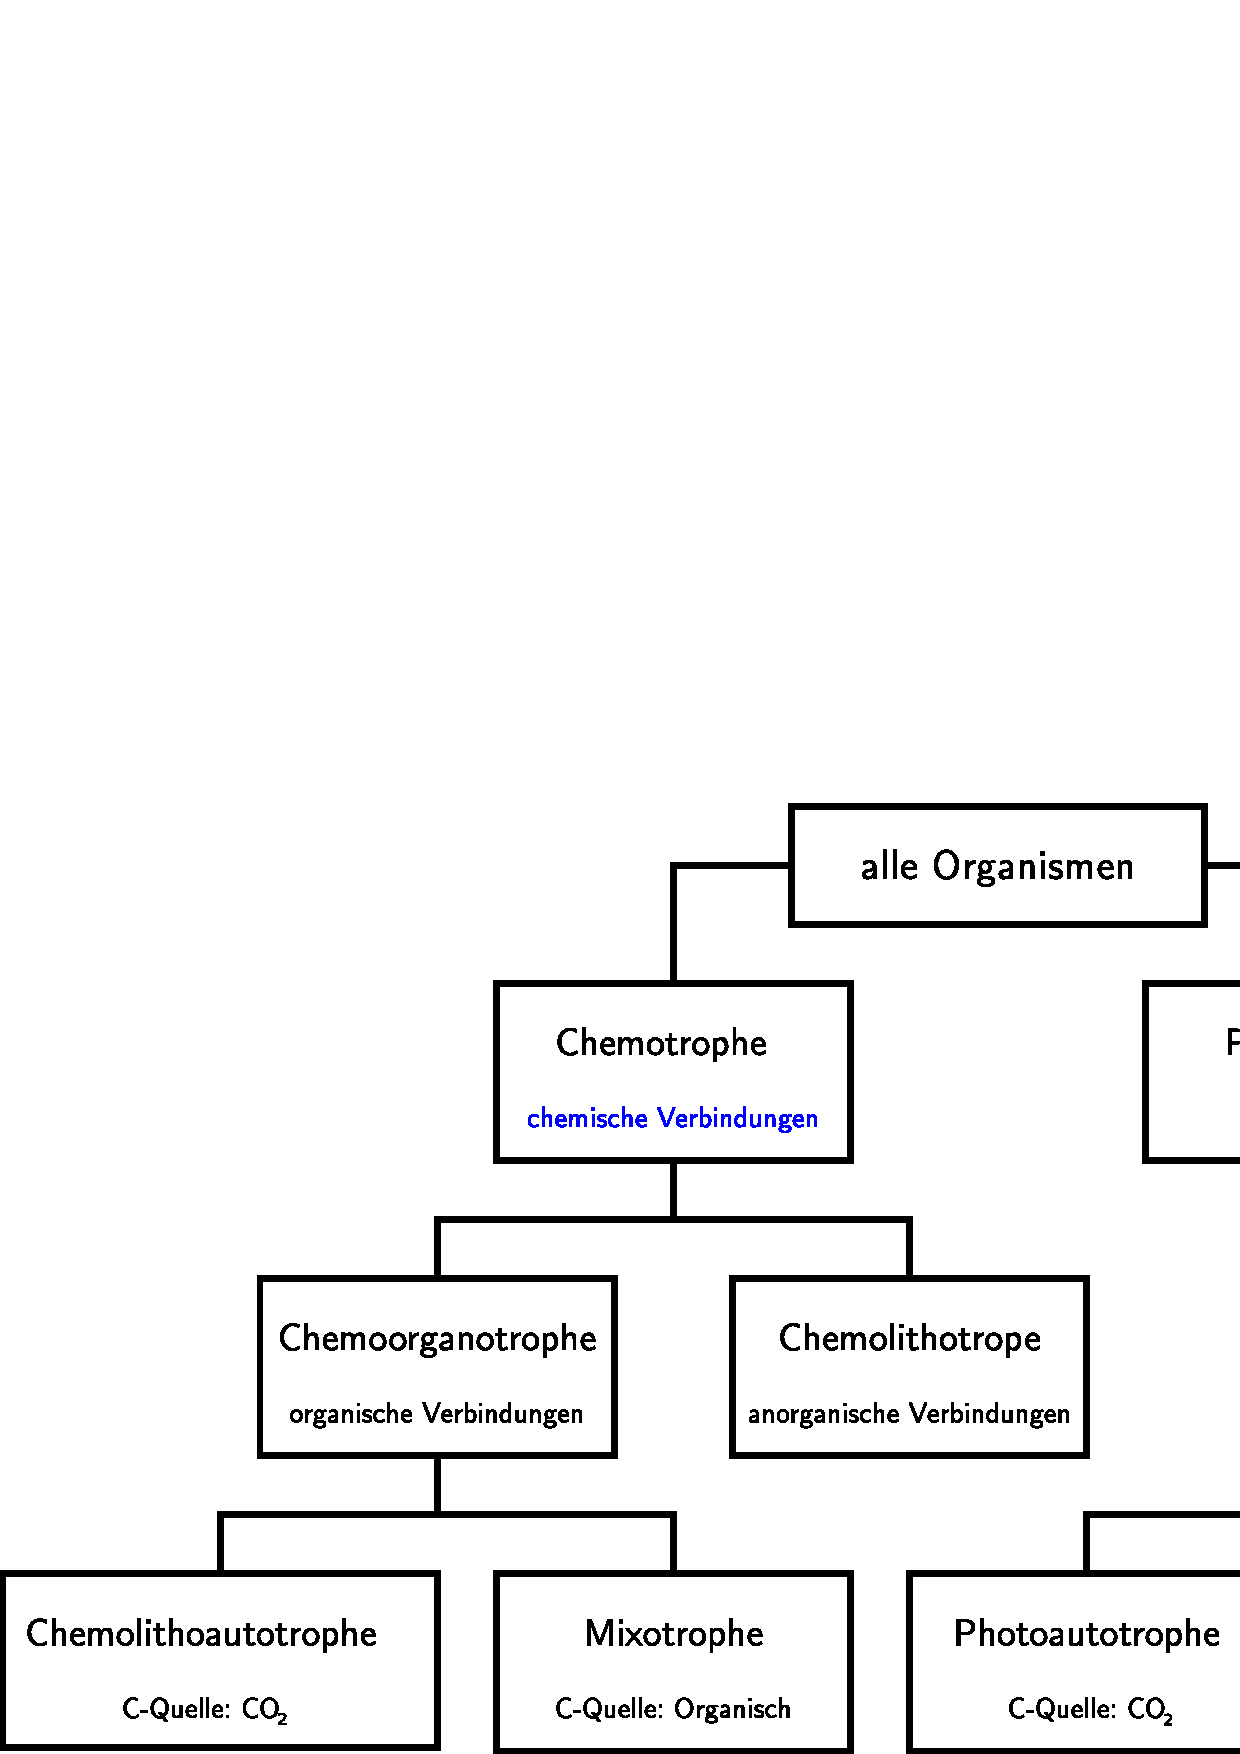
\includegraphics[scale=0.5]{./pictures/stoffwechsel.pdf}
		\end{center}
		\caption{\slshape{Stoffwechselvarianten von Mikroorganismen.
								Dargestellt sind die \textcolor{blue}{Energiequelle} und die Kohlenstoffquelle.}}
		\label{fig:Stoffwechselvarianten}
		\end{figure}

	\item[Substratkettenphosphorylierung]	\hfill	\\
		Bildung von ATP durch den direkten Transfer eines ernergiereichen
		Phosphatmoldeküls von einer phosphorylierten organischen Verbindung
		auf ADP.
\end{description}


\end{document}
\end{input}
